\section{Monday, 2/17: Feature selection, feature engineering, and regularization!}

We ended last class by talking about how both KNN and Linear Regression can do badly when the number of variables $p$ is very large! There are two distinct problems.
\begin{itemize}
\item For linear regression with no preprocessing, increasing $p$ just increases the model complexity of a linear regression model. This allows us to overfit (or memorize) our training set, which leads to very high variance and poor test error. 
\item For KNN, $p$ doesn't really have anything to do with model complexity, but we do poorly because KNN works best when we have training points that are dense in our feature space (so that the $k$ nearest neighbors to a test point $x$ are actually close to $x$). As $p$ grows, it is really really hard for points to be dense ($n$ would need to be HUGE), and so we are making predictions with neighbors that aren't really that close (bias) and who our neighbors actually are is affected by noise in so many different predictors (variance). 
\end{itemize}
Real data is high dimensional! So we really need a way around these issues! Today, we will talk about two strategies for avoiding issues with high dimensions.
\begin{itemize}
\item \textbf{Strategy 1: }	Preprocess the data to reduce the dimension before we apply the algorithm. Within strategy 1, we have two sub-strategies. 
\begin{itemize}
\item \textbf{Feature selection}: You have all used this for linear regression; it's a really natural fit. It definitely \emph{could} be used for KNN, but you would need to pick some sort of selection algorithm that might not have anything to do with KNN. 
\item \textbf{Feature extraction}: Can do this before KNN, linear regression, or any other algorithm. 
\end{itemize}
\item \textbf{Strategy 2: }	Modify the algorithm using \textbf{regularization} to automatically reduce the variance.
\begin{itemize}
\item We are going to talk about this in the context of linear regression, not KNN.
\item The concept (Regularization!!) will be relevant to any algorithm we use this semester that gets fit by minimizing a loss function. KNN is one of the only algorithms that we will use this semester that doesn't have this loss-function form, and so regularization is not directly applicable. 
\item It will turn out that Lasso regularization ends up looking a lot like variable selection! But they arise from slightly different concepts!
\end{itemize}
\end{itemize}

Let's talk about each of these! I am going to zoom through material today. Chapter 6 of ISL has a really nice treatment of feature selection, feature extraction, and regularization for linear regression. Please read this on your own!

\normalsize

\subsection{Feature selection}

The idea is that if we have $p$ predictors $\left\{X_j : j \in \{1,\ldots,p\}\right\}$ but we don't think that all of them are relevant, we should select a subset $\mathcal{S} \in \{1,\ldots,p\}$. We should then do our statistical learning algorithm using only $\left\{X_j : j \in \mathcal{S} \right\}$. If we do a good job with selection, we should improve our performance, because our variance will be smaller (for linear regression) and we will have less curse of dimensionality (for KNN).

\subsubsection{Guess and check}

You have all done variable selection for linear regression via what I might call ``guess and check" before. You have all fit a model with a bunch of variables, and then looked at the p-values and decided only to include variables that seem significant! You have also checked for things like multicollinearity, and removed variables that you are worried are redundant. All of these strategies are great, and show a big advantage of linear regression: we have interpretable tools for built-in variable selection. 

\subsubsection{Best subset regression}

A more automated way to do variable selection would be to try every single subset $\mathcal{S} \in \{1,\ldots,p\}$ and choose the subset that leads to the lowest test set MSE, the lowest AIC or BIC, or is the best according to some other metric.

If $p$ is small, we could just try out fitting least squares models to all of the different subsets $S \subset \{1,\ldots,p\}$. We could then directly compare our metrics for every possible subset, and if we pick the subset that leads to the lowest value we have our solution! This is best-subset regression, and I think you should have heard about it in Stat 346! Best-subset regression is kind of silly, because it is computationally infeasible when $p$ is big, which is exactly the situation in which we need it! 


\subsubsection{Forward stepwise regression}

Since best subset regression is computationally infeasible, one idea is to try to approximate the solution to best subset regression with a more reasonable  search strategy. With best subset regression, we would need to try out $2^p$ different models. With the forward stepwise algorithm suggested below, we need to try out at most $p+(p-1)+(p-2)+...$ models. 

The idea of forward stepwise regression is simple:
\begin{itemize}
\item Start with an empty model that only includes an intercept
\item Until a stopping criteria is met:
\begin{itemize}
\item Look through all possible predictors that are not yet in the model. Add the predictor that most improves the model at this moment! 
\end{itemize}	
\end{itemize}

We get to decide what we mean by ``most improves the model". We could, at each step, add the most significant predictor, or the one that most improves $R^2$, etc. We could use a stopping criteria such as: ``until the BIC stops improving" or ``until no variable that could be added has a p-value less than 0.05". If we do this, then the size of our final model is determined for us, using only the training set.

We could also use no stopping criteria, and just go until we run out of predictors, or until the number of predictors is equal to the number of datapoints. If we do this, we get a sequence of nested models, where the variables were added in a greedy order. We could select our final model size by seeing which of these nested models minimizes the test set error, for example. You did this on your homework. This idea of getting a whole sequence of models, and then selecting the one that minimizes test set error, will look a bit like regularization!

Note that backwards stepwise regression is also a thing that you may have learned about in Stat 346. I think it is unsatisfying when we are discussing high dimensional regression, since it cannot be used for $p > n$ (since you cannot fit the initial model to step backwards from). 

I think you all know a bit about feature selection for linear regression from Stat 346! So I will not talk too much more about it.

\subsubsection{Feature selection for KNN??}

KNN does not lend itself to a built-in way to do feature selection, as far as I know. We could ``try out fitting KNN with different features included or removed", and compare test MSE for different options. This is a lot like best-subset selection; it is computationally infeasible to try out all possible options. We could also run something like stepwise linear regression as a preprocessing step to KNN. This would be a strange thing to do, but the idea would be that we think we need wiggly functions (hence KNN), but we first want to have some efficient way to select variables that seem associated with $Y$. People also use a preprocessing method called marginal screening, which just computes the marginal correlation between $Y$ and $X_j$ for $j=1,\ldots,p$ and only keeps variables $j$ that seem correlated with $Y$. You could try this out with KNN! A fear with any of these methods is that removing some Xs can alter who is neighbors with who in your data: which might be good but it also might be bad!

\subsubsection{Overview:}

In general, what does feature selection get us, and what are the risks? 
\begin{itemize}
\item \textbf{Interpretability:} selecting a small number of features makes our final model more interpretable. 
\item \textbf{Usability:} A user needs to tune a hyper-parameter that controls "how many variables to keep." This makes everything a bit more complicated, but at least the tuning parameter is interpretable, and automated procedures exist. 
\item \textbf{Bias:} If we fail to include an important variable, we could introduce bias. In other words, we could accidentally select a model that is too simple. 
\item \textbf{Variance:} The whole point of feature selection is to reduce variance! It definitely does this. 
\item \textbf{Computational efficiency:} Some methods like best subset selection and stepwise regression could be slow. So the actual selection step can be slow. But in general, if we select only some features from our data and use these for the rest of our analyses, we have less data to store and we will make downstream tasks faster. 
\item \textbf{Inference:} If you were hoping that, after variable selection, you could get nice p-values from \texttt{lm()} for each of your selected variables, you are wrong! This is the problem of \emph{post-selection inference}, which is my research area! We cannot use the same data more model selection and model inference. If we want to do inference after model selection, we need to refit the selected model on a totally held-out test set. Ask me about this sometime, or do this topic for your final project! There are papers that do fancy math to do inference after stepwise regression!
\end{itemize}


\subsection{Feature extraction}

The idea is that if we have $p$ predictors $\left\{X_j : j \in \{1,\ldots,p\}\right\}$ but we think that a lot of them are redundant, maybe we can compress the information from the $p$ features into a smaller number of features $\left\{ \tilde{X}_k = f_k(\bold{X}) : k \in \{1,\ldots, S\} \right\}$. Each of the $S$ new features can contain information from all of the old features.  

Consider image classification. Our high-dimensional set of predictors is every pixel in an image. Feature selection will work terribly here: we can't just select some of the pixels for every image and expect to do a good job. But there are probably low-dimensional concepts hidden in the images that can capture all of the information that we need, without storing every single pixel. Thus, image classification is a setting where feature extraction is really helpful but where feature selection makes no sense.

Here are a few examples:

\begin{itemize}
\item The new features $\tilde{X}_k$ for  $k \in \{1,\ldots, S\}$ could be the first $S$ principal components of the original feature matrix $\bold{X}$. We still need to choose $S$: this is now a tuning parameter. 
\item It turns out that you can randomly project your original $p$-dimensional feature matrix $\bold{X}$ into a lower dimensional subspace to get $\tilde{X}$. Magical theorems say that the distances between observations are approximately preserved under random projections, and so this can work pretty well as a preprocessing step to KNN. 
\item PCA and random projections are linear embeddings. You could use something like UMAP or tSNE as a non-linear embedding. These are popular in genomics! They put your points onto a low-dimensional manifold. 
\item Autoencoders are a really cool way to learn a low dimensional representation of a high dimensional object! 
\end{itemize}

PCA is a really classic example, and I think that you are all familiar with PCA from Stat 346. I included a little sidebar on PCA below, just in case we have time to go over it or just in case you are curious. But how PCA actually works is not really our topic for today. 

The general idea of any of these is that we can avoid the curse of dimensionality if we can capture most of the information about our $\bold{X}$ variables in fewer dimensions. This is going to work best when we have a lot of redundant predictors. 

\subsubsection{PCA}

In the simplest case, if we assume that our feature matrix $X$ has been centered and scaled so that the mean of each variable is $0$ and the standard deviation of each variable is $1$, and we also assume that $n > p$, then we can take the singular value decomposition of $X$, and write it as 
$$
X = U D V^T, 
$$
where $U \in \mathbb{R}^{n \times p}$ is a matrix whose columns are orthogonal unit vectors, $D \in \mathbb{R}^{p \times p}$ is a diagonal matrix, and $V \in \mathbb{R}^{p \times p}$ is an orthonormal matrix. 

The columns of $V$ define a new set of axes in our predictor space. $V_1$ represents the direction that contains as much of the variance in $X$ as possible. $V_2$ represents the direction orthogonal to $V_1$ that explains as much of the leftover variance as possible, and so on. In PCA-speak, these are called the loadings. They correspond to the eigenvectors of the correlation matrix of the data $X$, and are ordered in such a way that $V_1$ corresponds to the biggest eigenvalue, $V_2$ to the second biggest eigenvalue, etc. 

If the columns of $V$ are the axes, then the columns of $U D$ store the position of each datapoint along these axes. We call these the scores. 

Let $U_{r}$ denote the first $k$ columns of $u$, let $D_r$ denote the first $r$ rows and columns of $D$, and let $V_r$ denote the first $r$ columns of $V$. Then, the matrix
$$
U_r D_r V_r^T, 
$$
is the ``best" (according to mean-squared-error or L2-norm) rank-r approximation to $X$. 

What this means is that if we let $\tilde{X} = U_r D_r \in \mathbb{R}^{n \times r}$, we have made ourselves $r$ new variables that store ``as much of the variation in $X$ as possible" (from a MSE perspective, and among linear embeddings). 

 The new variables are also independent of one another, so there is no multicollinearity left. We can use this $\tilde{X}$ in our downstream task. We probably only want to do this if it stores a large proportion of the total variance in $X$: we can plot this proportion of variance vs. $r$ to help decide how many principal components to keep! 



\subsubsection{Overview}

In general, what does feature extraction get us, and what are the risks? 
\begin{itemize}
\item \textbf{Interpretability:} Often, feature extraction can make a final model less interpretable. Occasionally, you can get lucky, and identify your top few principal components as recognizable concepts. 
\item \textbf{Usability:} You need to figure out how to extract features, how many PCs to keep, etc. This adds a tuning task that I think is less straightforward than the selection task. 
\item \textbf{Bias:} If you don't retain enough good information about $\bold{X}$, you could introduce bias. 
\item \textbf{Variance:} The point is to reduce variance! 
\item \textbf{Computational efficiency:} Story is the same as for feature selection. Something like UMAP is computationally hard to run, but it saves you time and space down the road because you don't need to store your entire high dimensional dataset anymore. 
\end{itemize}

One more nice thing is that something like PCA has nothing to do with linear regression. We can use PCA before KNN and it works really well: you will do this on your homework! So the techniques we use for feature extraction tend to be very general; even if Chapter 6 of your ISL textbook talks about PCA in the context of linear regression only. 


\subsection{Regularization}

The idea of regularization is to reduce our variance by adding a penalty on model complexity directly into our loss function!

\subsubsection{Best subset regression through L0-regularization!}

We can revisit the idea of best subset regression, but case it as a regularization problem. We can do linear regression, but we can let
\begin{equation}
\label{sparse}	
\hat{\beta} = \mathrm{argmin}_{b \in \mathbb{R}^p} \ \ \ \sum_{i=1}^n \left( y_i - x_i^T b \right)^2 + \lambda ||b||_0,
\end{equation}
where
$$
||b||_0 = \{ \#i : b_i \neq 0 \}.
$$
This is just saying that we want to fit a least squares regression, but we want to prefer a \emph{sparse} solution. 

The cool thing about writing the objective function in this way is that the parameter $\lambda$ directly controls the bias-variance tradeoff. If we set $\lambda$ to be very large, we will select a model with very few non-zero coefficients. This model will have a lot of bias (even if the *true* model is linear! because we might have accidentally left out important variables). However, the model will have low variance because it is so simple. On the other hand, as $\lambda$ approaches $0$, we approach our un-regularized high-dimensional regression, whose variance we know is very high. 

This is a nice idea! But there is one huge problem! Can we actually solve \eqref{sparse}? 

Unfortunately, the answer is no! Not efficiently! The only way to solve \eqref{sparse} exactly is to try out all $2^p$ possible models, which is infeasible. While this first example of regularization is not actually something that we do in practice, the idea turns out to be really useful!  

\subsubsection{Ridge regression through L2-regularization!}

One reason that we cannot solve \eqref{sparse} is that our favorite way to find minimums is to take a derivative, and $||b||_0$ is not differentiable. So, what if we just modified  \eqref{sparse} to make it differentiable? Ridge regression solves the following optimization problem:
\begin{equation}
\label{ridge}	
\hat{\beta} = \mathrm{argmin}_{b \in \mathbb{R}^p} \ \ \ \sum_{i=1}^n \left( y_i - x_i^T b \right)^2 + \lambda ||b||_2^2,
\end{equation}
where
$$
||b||_2^2 = \sum_{i=1}^p b_i^2. 
$$
Unlike \eqref{sparse}, we can solve \eqref{ridge} in closed-form. You will do this on HW2! But ... what does it get us?\\
\\
If, in truth, $y_i = x_i^T \beta + \epsilon$, then the solution to  \eqref{ridge} is biased for $\beta$. The amount of bias will grow as $\lambda$ grows. However, we can prove that, as $\lambda$ grows, the variance of the solution to \eqref{ridge} always goes down. So, while the least squares solution ($\lambda=0$) is known to be the Best Linear Unbiased Estimator, it turns out that some solutions to \eqref{ridge} (i.e. solutions for some other values of $\lambda$) could have lower expected prediction error than the least squares solution--- even though they are biased! This is really cool- but how do we find these $\lambda$s? \\
\\
We have not officially talked about K-fold cross-validation yet in this class. While it is a really general technique that has nothing to do specifically with ridge regression, I am going to talk about it right now! Because it is the way we will choose a value of $\lambda$ for ridge regression. \\
\\
Here is how we would use K-fold cross-validation in this context! 
\begin{itemize}
\item Divide our $n$ datapoints into $K$ non-overlapping folds of data. 
\item For $k$ in $1,\ldots,K$:
\begin{itemize}
\item Let the $k$th fold be the test set. Let the other $K-1$ folds be the training set. 
\item For $\lambda'$ in a big grid of possible values of $\lambda$:
\begin{itemize}
\item Solve \eqref{ridge} with $\lambda=\lambda'$, using the training set. 
\item Compute the prediction error on the test set. Save this error for this fold and this value $\lambda'$. 
\end{itemize}
\end{itemize}
\item For each $\lambda'$, add up the test set errors across all $K$ folds.
\item Select the $\lambda^*$ that minimizes the total test set error. \emph{(Or use the 1-SE rule to select a slightly different $\lambda^*$. We will come back to this at some point on a HW.)}
\item Refit \eqref{ridge}, using all $n$ datapoints and $\lambda^*$. Let this be your final model. 
\end{itemize}

Ok, so we know that we can solve \eqref{ridge}. And we also know that we can use cross validation to pick a $\lambda^*$ that hopefully hits a sweet spot of bias and variance. There are a few practical notes to talk about.
\begin{itemize}
\item It is good to center and scale your $X$ variables before you apply ridge. The reason you should center them is that we want our model to spiritually include an intercept, but we don't want to put the penalty $\lambda$ on the intercept. It is good to scale them because we don't want a variable with different units to get unfairly penalized by the penalty term- we want all of the coordinates of $b_i$ to be on the same scale. 
\item The solution to \eqref{ridge} is not sparse, so is not necessarily interpretable. Sometimes, people look at the output of \eqref{ridge} and look at which variables got their coefficients shrunken very small. They then decide to remove those, and refit a final model using least squares to only the remaining variables. This makes the final model more interpretable. We should note that standard ``lm()`` based inference is  invalid after doing this (it's the same issue as doing inference after variable selection). 
\item The amount by which the ridge solution shrinks each element of $\hat{\beta}$ actually depends on the singular vectors of $X$! Which is cool! More redundancy in the columns of $X$ will lead to more shrinkage. This makes sense, because we also know that more redundancy in the columns of $X$ means more variance in a least squares solution, so more shrinkage is needed!
\item There are a lot of cool things we could study for ridge. It's mathematically beautiful! For example, there is a way to view ridge regression as a continuous analog of regression in principal components! That is so cool. A few cool things about ridge will be on your HW or in the textbook. For now, we will move on!
\end{itemize}

\subsubsection{Lasso regression through L1 regularization}

It is sort of a bummer that ridge regression does not give us sparse solutions. It does reduce the variance of the fitted model, but just by looking at the fitted model it is hard to tell that we have reduced its complexity. That is where lasso comes in. Magically, it turns out that the solution to
\begin{equation}
\label{lasso}	
\hat{\beta} = \mathrm{argmin}_{b \in \mathbb{R}^p} \ \ \ \sum_{i=1}^n \left( y_i - x_i^T b \right)^2 + \lambda ||b||_1,
\end{equation}
where
$$
||b||_1 = \sum_{i=1}^p | b_i |,
$$
tends to be sparse! We call this Lasso regression! 

A lot of things are the same as with ridge. The parameter $\lambda$ governs a bias-variance tradeoff. You should be sure to center and scale your variables before you use Lasso. You should use cross validation to select the best value of $\lambda$. 

By sparse, we mean that, for large enough $\lambda$, all of the coefficients will be shrunk towards $0$, but several will be exactly $0$. This means that the Lasso actually performs variable selection! This is such a simple change compared to \eqref{ridge}. Why would the solution suddenly be sparse? This is a fun optimization fact that is often explained using Figure~\ref{fig_lassoridge}. 

Of course, an issue is that $||b||_1$ is no longer differentiable. In fact, this is a non-convex optimization problem. So, while Ridge had a closed-form solution, Lasso does not. We need to solve \eqref{lasso} with an iterative algorithm called coordinate descent.

In a setting where all variables are actually related to the response variable, Ridge regression tends to have slightly better test set performance than Lasso (at their respective optimal values of $\lambda$, which do not need to be the same). However, in a setting where the true solution is sparse, Lasso can outperform ridge. So, in practice, both are useful tools, and you might want to compare them for a given problem using cross validation. Personally, I love the  Lasso because I love the sparse property for interpretability. But some problems are not sparse! (Remember our image example!). 

Note that, if you are using Lasso for variable selection, you might want to handle categorical dummy variables in a special way. You might want to make sure that groups of $\beta$s representing categories of the same variable are either selected or not selected together. You can do this with the group-lasso. 







\begin{figure}
\centering
	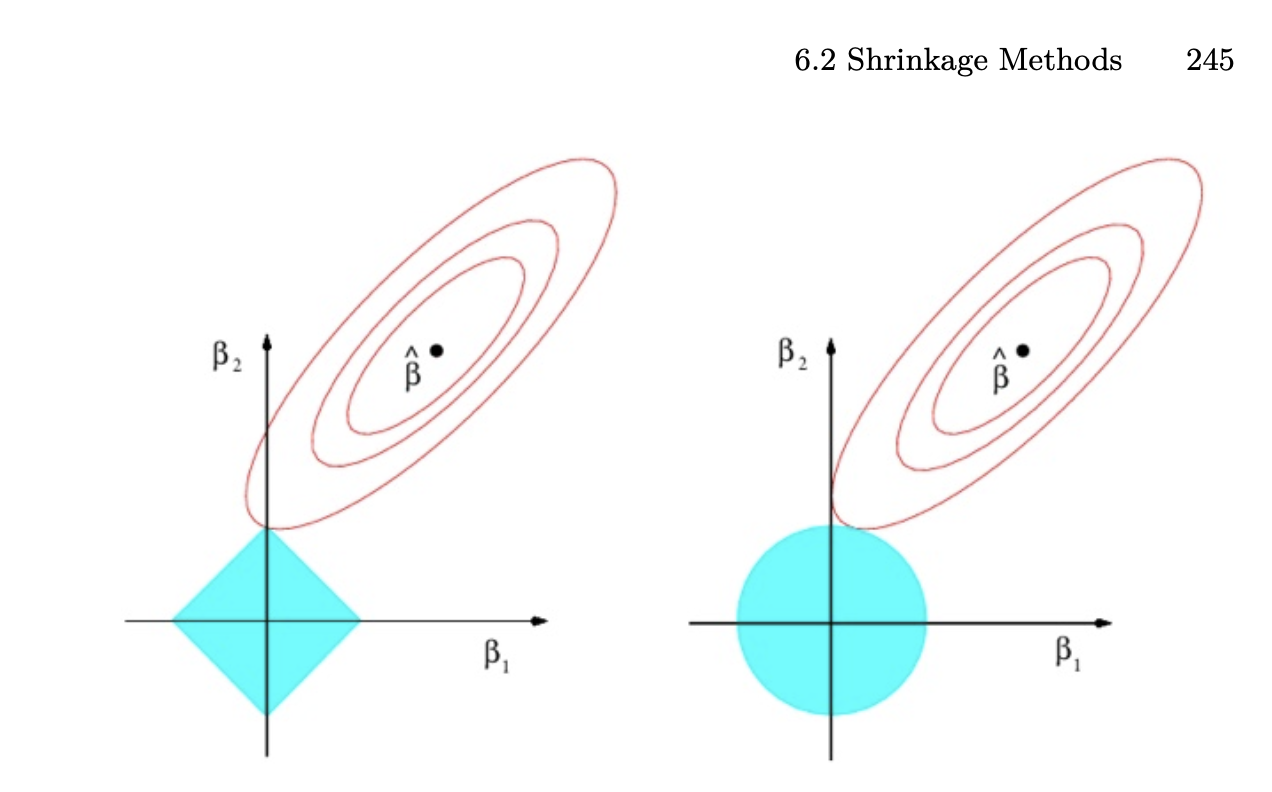
\includegraphics[width=0.7\textwidth]{442_lecs/magicpic.png}
	\caption{A figure taken from ISL that illustrates why the Lasso prefers sparse solutions while Ridge does not. If we are optimizing the least squares objective (oval) subject to the constraint that either the L1 or L2 norm of $\beta$ is not too large, the our solution will lie in the place where the contours of our least squares objective first hit our constraint set. For the L2 constraint (circle), this can happen anywhere. For the L1 solution (diamond), this is more likely to happen on one of our 4 pointy corners.}
	\label{fig_lassoridge}
\end{figure}


\subsubsection{Overview}

In general, what does regularization get us, and what are the risks?

\begin{itemize}
\item We will work with so many algorithms this semester that can be written as: ``minimize this loss function over a training set". Any algorithm that has this form has the risk of overfitting to the training set! But adding regularization on model complexity can always help us avoid overfitting! This is beautiful and general!
\item \textbf{Usability:} We need to do cross validation to choose $\lambda$. Luckily, for things like Ridge and Lasso, this is really easy and is just built into the software. 
\item \textbf{Bias:} Regularization introduces bias.
\item \textbf{Variance: } Regularization reduces variance. That is the whole point!
\item \textbf{Computational efficiency vs. interpretability: } From an interpretability standpoint, we most would have wanted to do L0 regularization. This encourages sparse solutions, but doesn't actually shrink the values of coefficients that are in our model. However, L0 regularization is computationally infeasible. On the other hand, L2 regularization is really fast and efficient, but the solution is not sparse and so isn't as interpretable. L1 regularization is a nice happy medium! It does not have a closed form solution but we can still solve it, and we get a sparse solution (with coefficients that also got shrunk). 
\end{itemize}


\subsection{Wrap up}

I am sure I forgot some key points and I am sure we will be rushed! We will do our Lasso/Ridge R demo next class, and use that as a way to revisit some points! \\
\\
In general, even if Ridge and Lasso got smushed into one lecture in this class, I hope that you will remember them forever! They are really fundamental concepts! We have ridge/lasso logistic regression too- it's not only a linear regression thing! It's a really beautiful example of the bias-variance tradeoff and the interplay between optimization and statistics!

\section{Thursday, 2/20: Wrap up regularization, introduction to classification}

\subsection{Wrap up from last time}

...

\subsection{What is classification}

We are switching gears! We assume that we still have a setup with $n$ observations, $p$ predictors in $X$, and one response variable $y$. But now we assume that $y$ is a categorical variable! 

We still believe that there is some \emph{true} data generating process that generates $y$ from $X$, with some noise. However, it may not make sense anymore to write $y = f(X) + \epsilon$. Because, if $y$ is a category, what form does the noise $\epsilon$ take on?

To study this \emph{classification} problem, we need some new language! 

Let's start where the simplest case where there are only two possible categories for $y$, and for simplicity, let's encode them as $0$ and $1$. If we think that $y_i$ is related to $x_i$, but that there is also some random noise in $y_i$, then the reasonable thing to do is to model: 
$$
Y_i \mid X_i \sim \mathrm{Bernoulli}\left( f(X_i) \right). 
$$
The idea once again is that $f()$ is some true, unknown function. We really want to estimate $f()$: either just because we want to make good predictions in the future, or because we want to understand and interpret which predictors $X$ are most contributing to $Pr(Y_i=1)$. 


%\begin{itemize}
%\item What is classification? How do we evaluate a classifier?
%\item The Bayes classifier
%\item Review of logistic regression.
%\item The ROC curve. 
%\end{itemize}



